\section{INS Equations}
In this section, we will derive the INS equations.
\subsection{Euler Angles}
\[
R_m = \dfrac{a(1-e^2)}{(1-e^2\sin^2\phi)^{3/2}}
\]
\[
    R_p = \dfrac{a}{(1-e^2\sin^2\phi)^{1/2}}
\]
\[
    R_g = \sqrt{R_m R_p}
\]
$F_b$ is the measured force on the body.
$\omega_{ib}^b$ is the angular velocity of the body with respect to the inertial frame, expressed in the body frame that is measured by the gyroscope.
\[
    \omega_{ie}^n = \begin{bmatrix}
        \Omega_e \cos\phi \\
        0 \\
        -\Omega_e \sin\phi
    \end{bmatrix}
\]
\[
    \omega_{en}^n = \begin{bmatrix}
        \dfrac{v_e}{R_p+h} \\[1em]
        -\dfrac{v_n}{R_g+h} \\[1em]
        -\dfrac{v_e\tan\phi}{R_p+h}
    \end{bmatrix}
\]
\[
    \omega_{in}^n = \omega_{ie}^n + \omega_{en}^n
\]
\[
    \bm{C}_n^b = \begin{bmatrix}
        \cos\theta\cos\psi & \cos\theta\sin\psi & -\sin\theta \\
        -\cos\phi\sin\psi+\sin\phi\sin\theta\cos\psi & \cos\phi\cos\psi+\sin\phi\sin\theta\sin\psi & \sin\phi\cos\theta \\
        \sin\phi\sin\psi+\cos\phi\sin\theta\cos\psi & -\sin\phi\cos\psi+\cos\phi\sin\theta\sin\psi & \cos\phi\cos\theta
    \end{bmatrix}
\]

\[
    \omega_{nb}^b = \omega_{ib}^b - \bm{C}_n^b \omega_{in}^n
\]

\[
    \begin{bmatrix}
        \dot{\phi} \\
        \dot{\theta} \\
        \dot{\psi}
    \end{bmatrix} = \begin{bmatrix}
        1 & \sin\phi\tan\theta & \cos\phi\tan\theta \\
        0 & \cos\phi & -\sin\phi \\
        0 & \dfrac{\sin\phi}{\cos\theta} & \dfrac{\cos\phi}{\cos\theta}
    \end{bmatrix} \omega_{nb}^b
\]
Acceleration of the body in the inertial frame:
\[
    F_n = \bm{C}_b^n F_b
\]
Gravity in navigation frame:
\[
    g_n = \begin{bmatrix}
        0 \\
        0 \\
        9.780318(1+0.0053024\sin^2\phi-0.0000058\sin^2(2\phi)) - 0.000003085h
    \end{bmatrix}
\]
\[
    \dfrac{g_n}{(1 + h/R_g)^2} 
\]
correction terms:
\[
    (2\omega_{ie}^n + \omega_{en}^n) \times V
\]

\[
    F = F_n + F_g - (2\omega_{ie}^n + \omega_{en}^n) \times V
\]

\[
    \dot{V} = F
\]

\[
    \bm{C}_e^n = \begin{bmatrix}
        \cos\phi & -\sin\phi\sin\lambda & \sin\phi\cos\lambda \\
        0 & \cos\lambda & \sin\lambda \\
        -\sin\phi & -\cos\phi\sin\lambda & \cos\phi\cos\lambda
    \end{bmatrix}
\]
\[
    \dot{\bm{C}}_e^n = -\tilde{\omega}_{en}^n\bm{C}_e^n
\]
Calculating position from $\bm{C}_e^n$:
\[
    \phi = \arcsin(C_{31})
\]
\[
    \lambda = \arctan2(-C_{32}, C_{33})
\]
Second solution for the position:
\[
    \dot{\phi} = \dfrac{v_n}{R_m+h}
\]
\[
    \dot{\lambda} = \dfrac{v_e}{(R_p+h)\cos\phi}
\]

The results are shown in the below figures.
\begin{figure}[H]
    \centering
    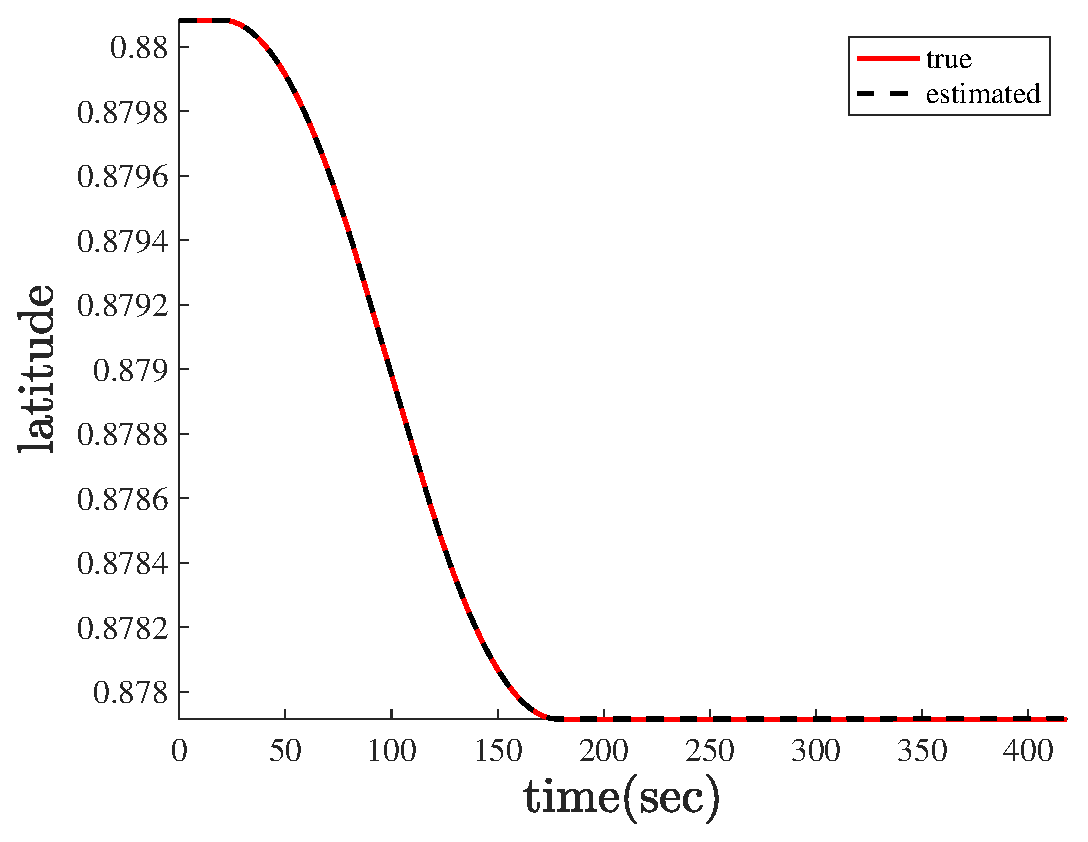
\includegraphics[width=0.7\textwidth]{../Figure/Q5/latitude}
    \caption{Latitude}
\end{figure}
\begin{figure}[H]
    \centering
    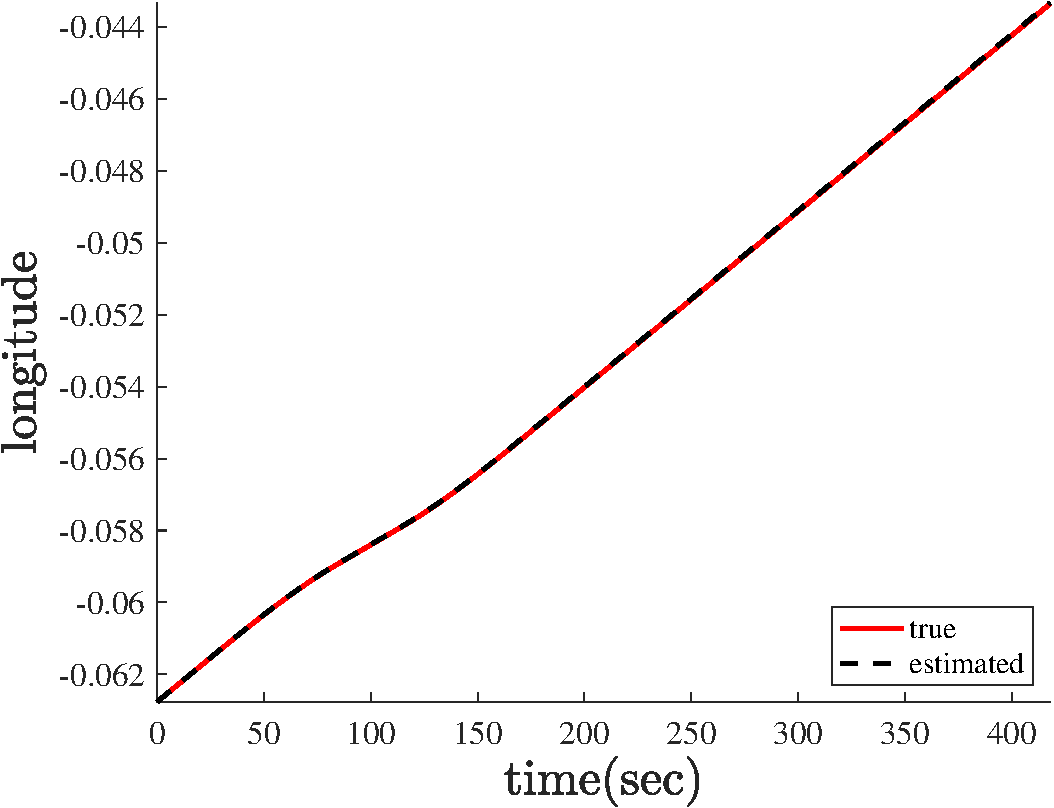
\includegraphics[width=0.7\textwidth]{../Figure/Q5/longitude}
    \caption{Longitude}
\end{figure}
\begin{figure}[H]
    \centering
    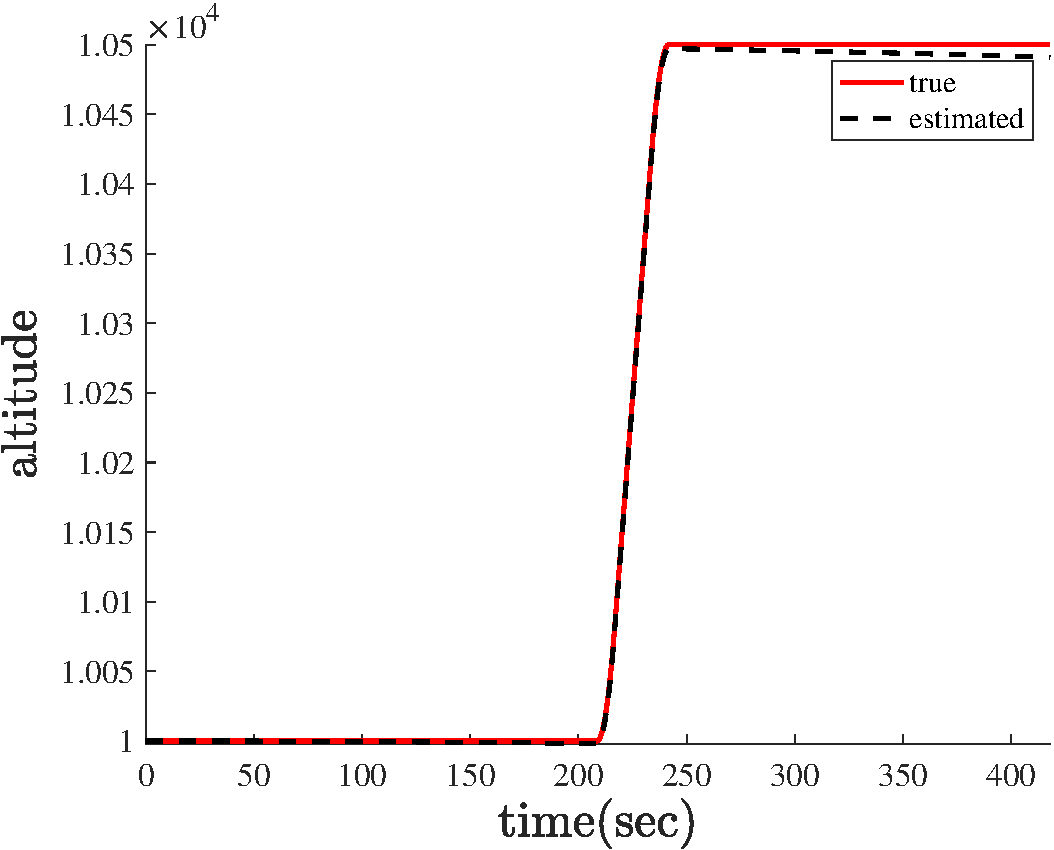
\includegraphics[width=0.7\textwidth]{../Figure/Q5/altitude}
    \caption{Altitude}
\end{figure}
\begin{figure}[H]
    \centering
    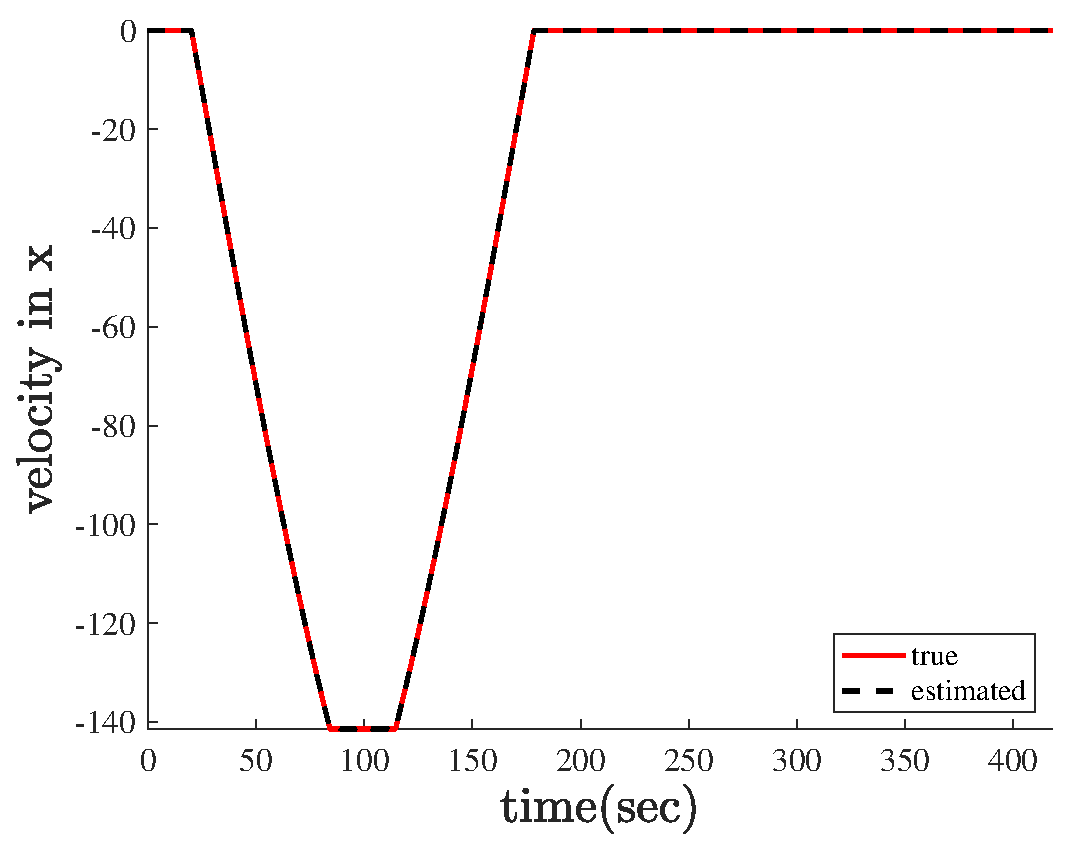
\includegraphics[width=0.7\textwidth]{../Figure/Q5/velocity_x}
    \caption{Velocity in x direction}
\end{figure}
\begin{figure}[H]
    \centering
    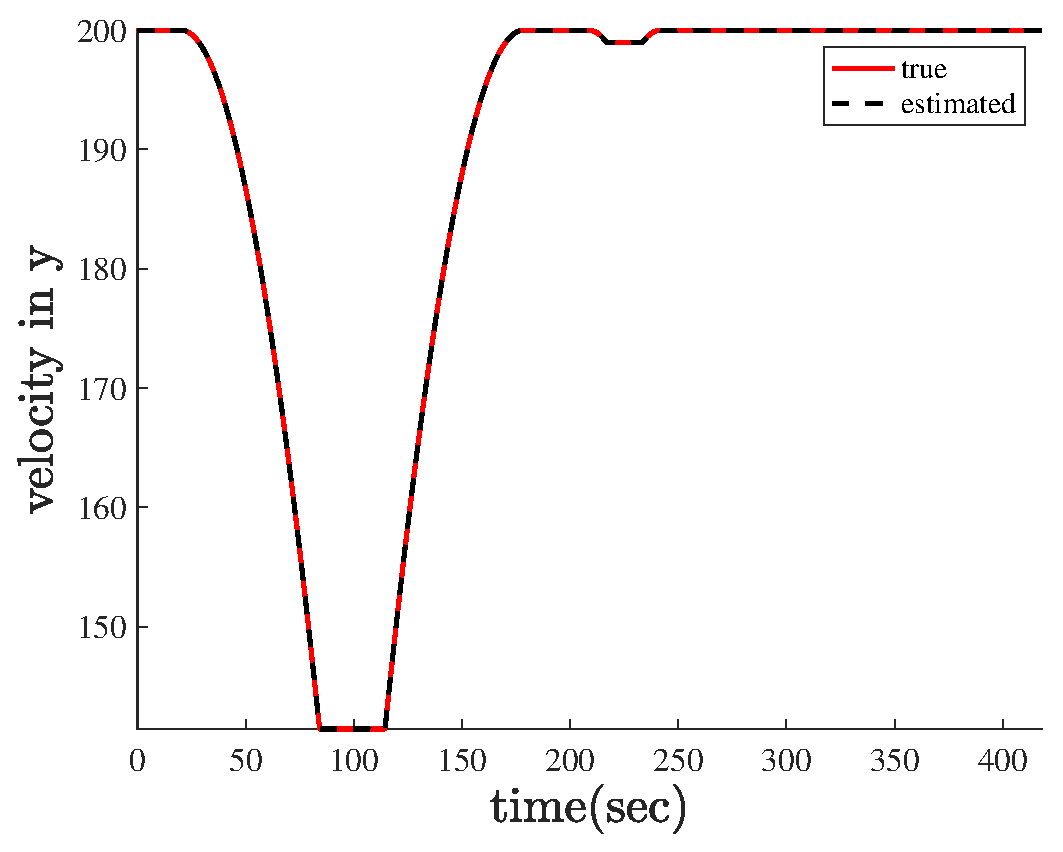
\includegraphics[width=0.7\textwidth]{../Figure/Q5/velocity_y}
    \caption{Velocity in y direction}
\end{figure}
\begin{figure}[H]
    \centering
    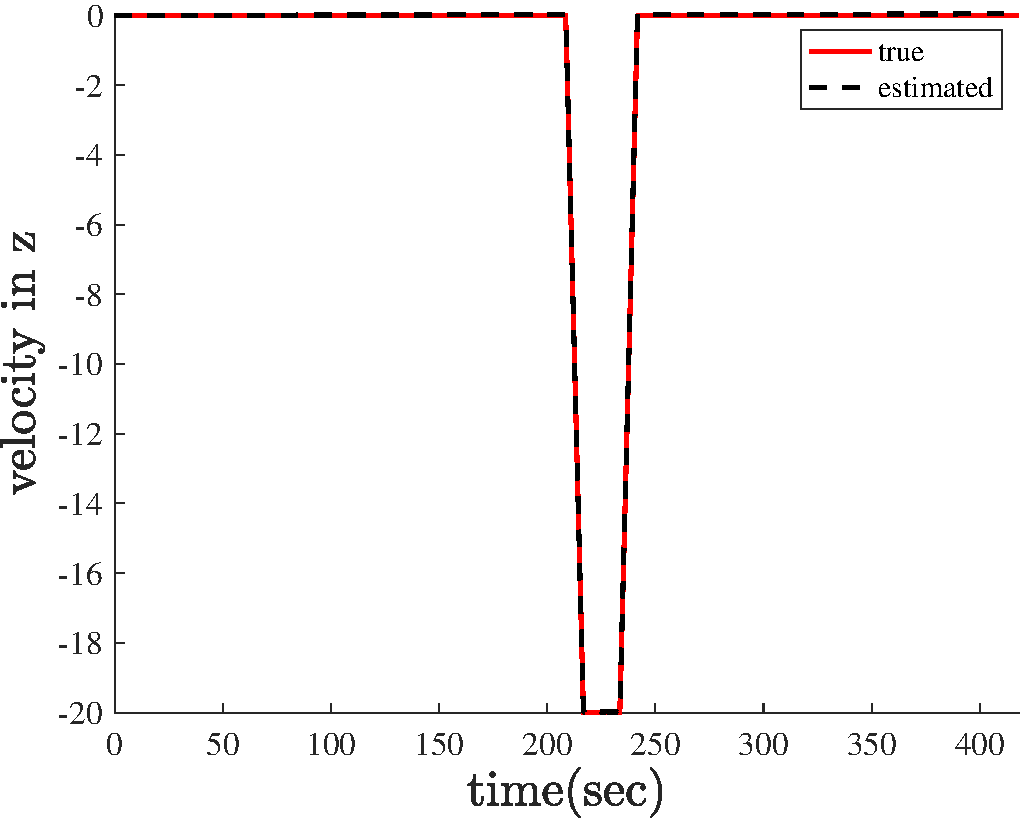
\includegraphics[width=0.7\textwidth]{../Figure/Q5/velocity_z}
    \caption{Velocity in z direction}
\end{figure}

\begin{figure}
    \centering
    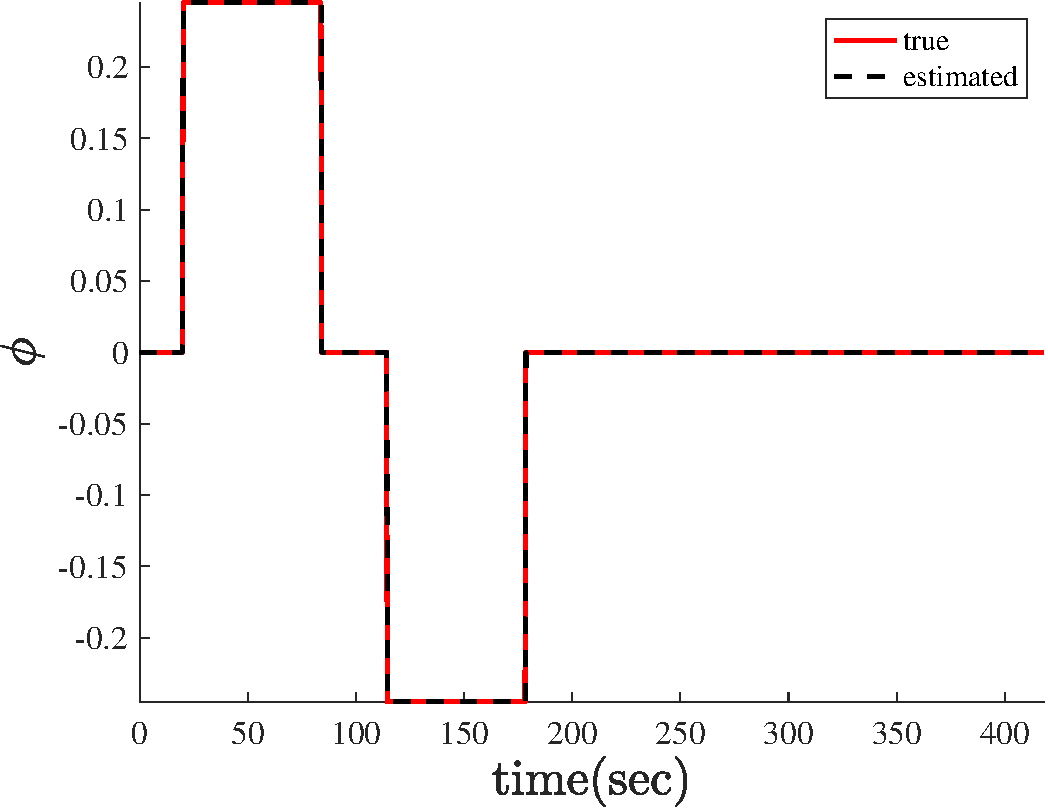
\includegraphics[width=0.7\textwidth]{../Figure/Q5/phi}
    \caption{Roll}
\end{figure}
\begin{figure}
    \centering
    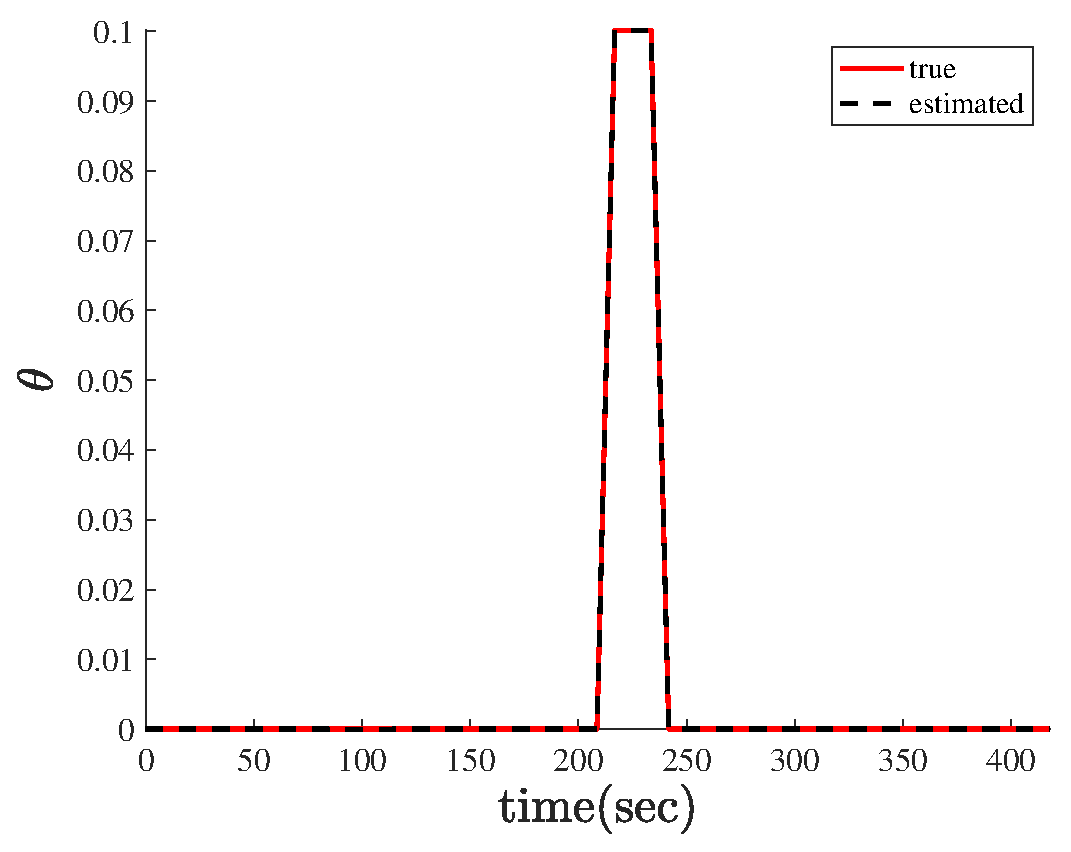
\includegraphics[width=0.7\textwidth]{../Figure/Q5/theta}
    \caption{Pitch}
\end{figure}
\begin{figure}
    \centering
    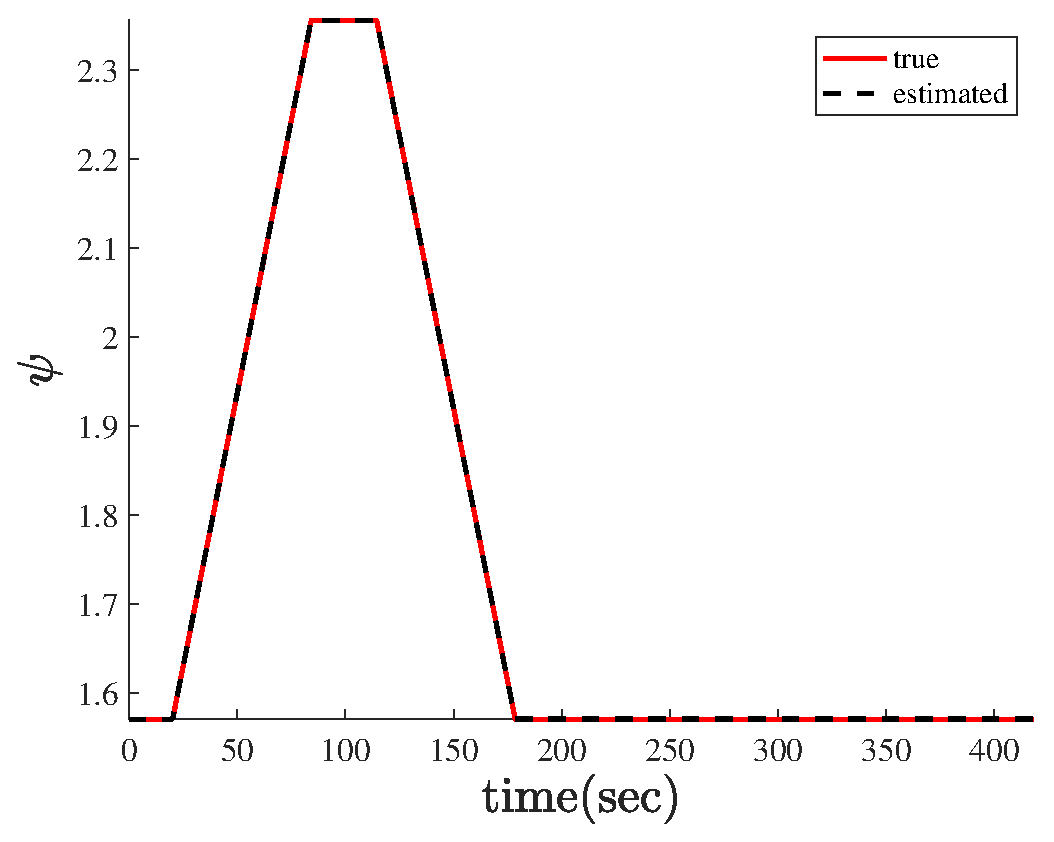
\includegraphics[width=0.7\textwidth]{../Figure/Q5/psi}
    \caption{Yaw}
\end{figure}